\documentclass[a4paper, 11pt]{article}

\usepackage[top=2cm, bottom=2cm, left=2cm, right=2cm]{geometry}
\usepackage[utf8]{inputenc}
\usepackage[T1]{fontenc}
\usepackage[frenchb]{babel}
\usepackage{textcomp}

\usepackage[usenames,dvipsnames]{xcolor}

\usepackage{hyperref}
\hypersetup{
	colorlinks=true,       	% false: boxed links; true: colored links
	linkcolor=black,          	% color of internal links
	urlcolor=blue,           	% color of external links
	citecolor=blue
}

\usepackage{listings}
\definecolor{dkgreen}{rgb}{0,0.6,0}
\definecolor{gray}{rgb}{0.5,0.5,0.5}
\definecolor{mauve}{rgb}{0.58,0,0.82}
\definecolor{blue}{rgb}{0,0,0.7}
\lstset{
	language=Matlab,
	basicstyle=\scriptsize,
	numbers=left,                   % where to put the line-numbers
  	numberstyle=\tiny\color{gray},
	commentstyle=\color{dkgreen},
	frame=single,                   % adds a frame around the code
 	rulecolor=\color{black},
	emph={},
	emphstyle=\color{mauve},
	morekeywords={},
	keywordstyle={\color{blue}},
	showstringspaces=false,
  	tabsize=4
}

\usepackage{framed}
\definecolor{shadecolor}{rgb}{0.96,0.96,0.96}

\usepackage{dashrule}
\usepackage{wrapfig}
\usepackage{graphicx}
\usepackage{enumitem}
\usepackage{wrapfig}
\usepackage{cancel} % diagonal strikeout
\usepackage[margin=1cm]{caption}
\usepackage{subcaption}
\setdescription{leftmargin=1cm,labelindent=0.5cm}

\usepackage{amsmath}
\usepackage{amsfonts}
\newcommand\mathd[0]{\mathrm{d}}

\usepackage{blindtext}

\title{PR202 - Rapport \\
\normalsize{Groupe 3}}
\date{\today}

\begin{document}
\maketitle

\newpage
\tableofcontents

\newpage

\section{Introduction}
L'unité PR202 s'inscrit dans la continuité de l'unité EL202. Ce projet nous demande de réaliser un jeu vidéo en VHDL jouable sur un écran VGA. Les objectifs sont nombreux. Techniquement, il nous permet d'améliorer notre connaissance du VHDL, de comprendre les bases de l'utilisation du VGA et de l'interfacage d'autre périphériques. Il nous introduit également aux protocoles liés au matériel. Ce projet est également l'occasion pour nous de perfectionner notre connaissance de la gestion de projet et d'avoir une autre expérience de la division du travail.\\

Notre trinôme a choisi de réaliser un PONG. Ce jeu vidéo développé par Atari en 1972 est le jeu qui a lancé l'industrialisation du jeu vidéo. Initialement sorti sous la forme d'une borne d'arcade, il donne vite naissance à une console dédiée \cite{cite:pong}.\\

\begin{figure}[h!]
	\centering
	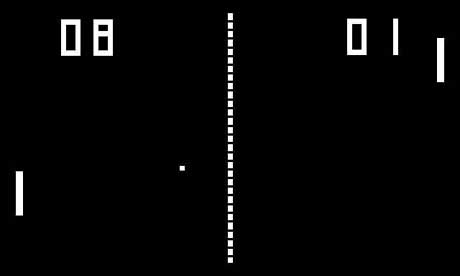
\includegraphics[scale=0.75]{images/pong.jpg}
	\caption{Capture d'écran de PONG (1972)}
	\label{fig:pong}
\end{figure}

\newpage

\section{Théorie}
\subsection{Video Graphics Array (VGA)}
Le VGA (Video Graphics Array) est un standard qui à l'origine a été développé pour l'affichage sur des écrans CRT (Cathode Ray Tube). Un écran à tube cathodique contient un canon à électrons dont le rayon balaye l'écran phosphorescent et produit de la lumière au contact de ce dernier. Le mouvement de balayage est réalisé grâce à des bobines produisant des champs magnétiques dans le tube, une paire de bobines permet le balayage horizontal et l'autre paire permet le balayage vertical. Dans le cas d'un tube couleur, celui-ci possède trois canons à électrons dont les rayons vont passer par un masque (Shadow mask ou masque utilisé sur tube Trinitron) afin d'afficher la couleur souhaitée.\\

Le standard VGA est également disponible sur les écrans LCD, et bien que la technologie soit différente, le comportement d'un écran CRT est reproduit. Le principe d'affichage reste donc le même dans les deux cas.\\

\begin{figure}[h!]
	\centering
	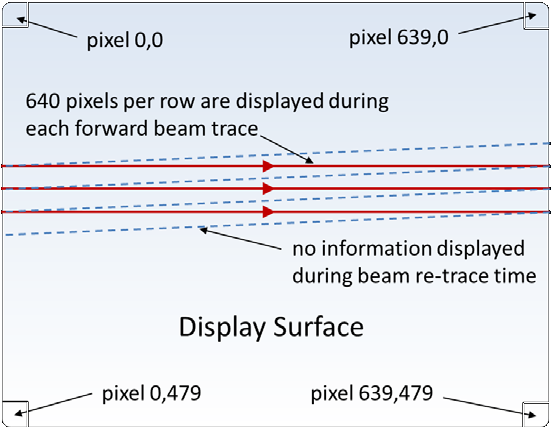
\includegraphics[scale=0.6]{images/scan.png}
	\caption{Balayage de l'écran \cite{cite:scan}}
	\label{fig:scan}
\end{figure}

L'écran est balayé de gauche à droite et de bas en haut, afin d'afficher une couleur pixel par pixel. Une fois le rayon arrivé en fin d'une ligne ou en bas à droite de l'écran, des temps d'attentes sont introduits, en effet dans le cas d'un tube cathodique cela s'expliquait par le temps nécessaire au tube pour revenir en début de ligne ou début d'écran (pixel en haut à gauche).\\

\begin{figure}[h!]
	\centering
	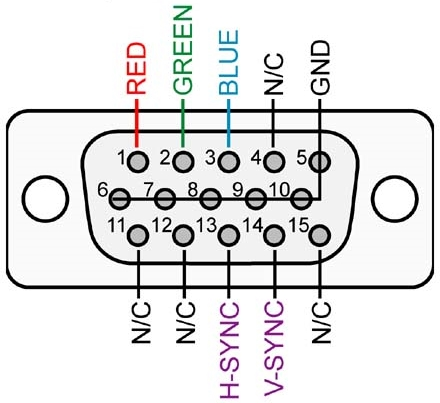
\includegraphics[scale=1.0]{images/vgapinout.jpg}
	\caption{Connecteur VGA mâle \cite{cite:vgapinout}}
	\label{fig:vgapinout}
\end{figure}

\newpage
Le connecteur VGA possède 15 pins (connecteur D-SUB 15-pin), 3 pins sont utilisés pour les signaux de couleurs (rouge, vert et bleu), 1 pin est utilisé pour la masse et 2 pins correspondent aux signaux de synchronisation \emph{hsync} et \emph{vsync}.\\

Parmi les signaux à produire listés ci-dessus, des signaux correspondent aux couleurs primaires rouge, vert et bleu. Ces signaux possèdent une tension comprise entre 0 et 0.7 volts et permettent, pour un pixel donné de déterminer sa couleur finale. Une couleur est une information qui peut être codée sous forme de signal numérique sur plusieurs bits.

\begin{snugshade}
\noindent \textbf{Exemple}: si le rouge est codé sur 3 bits, le vert sur 3 bits, et le vert sur 2 bits, il y aura alors $2^8 = 256$ possibilités de couleurs pour un pixel donné.
\end{snugshade}

\noindent Cette information numérique nécessite d'être convertie en signal analogique afin de pouvoir être exploitée par l'écran. En effet, les signaux de couleurs possèdent une tension que nous souhaitons faire varier afin de modifier l'intensité des couleurs. Pour convertir une information numérique en signal analogique, nous avons besoin d'un convertisseur numérique analogique (DAC). Ci-dessous le schéma d'un DAC 3 bits pour la couleur rouge et le calcul associé donnant la tension de sortie avec ce choix de résistances pour les 3 entrées à l'état haut.\\

\begin{multicols}{2}
	\noindent
	\begin{minipage}{\linewidth}
		\centering
		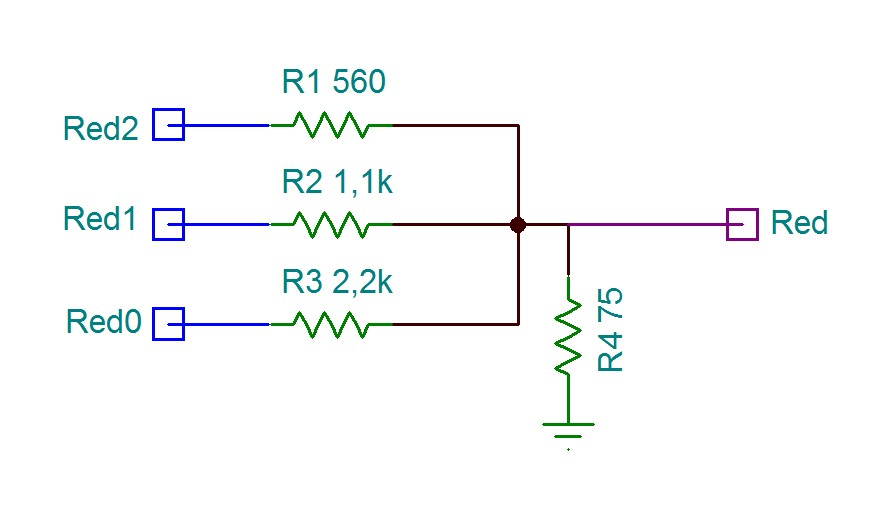
\includegraphics[scale = 0.25]{images/simple_dac.jpg}
		\captionof{figure}{VGA timing \cite{cite:psocvga}}
		\label{fig:vgadac}
	\end{minipage}
	
	\begin{flalign*}
	V_{red} = &\frac{\frac{3.3}{560} + \frac{3.3}{1100} + \frac{3.3}{2200}}{\frac{1}{560} + \frac{1}{1100} + \frac{1}{2200} + \frac{1}{75}}&\\
			= &0.63 V&
	\end{flalign*}
\end{multicols}

Les signaux \emph{hsync} et \emph{vsync} sont respectivement les signaux de synchronisation horizontale et verticale. Ce sont tous deux des signaux actifs à l'état bas. Le signal \emph{hsync} devient actif lorsqu'une ligne a été parcourue et que le canon à électrons doit se repositionner au début de la ligne suivante. Le signal \emph{vsync} devient actif lorsque le dernier pixel a été atteint en bas à droite de l'écran et que le canon à électrons doit se repositionner au début de l'écran (en haut à gauche). Les deux signaux de synchronisation sont actifs pendant une durée \emph{sync pulse} qui elle même est entourée par une durée \emph{back porch} et une durée \emph{front porch}. Ces durées sont différentes pour le parcours horizontal et vertical de l'écran, et dépendent également de la résolution choisie ainsi que la fréquence de rafraîchissement de l'écran. De plus, la fréquence à laquelle l'écran doit être parcouru dépend également de ces informations.
\begin{snugshade}
\noindent \textbf{VGA 640 x 480 60 Hz \cite{cite:timingsvga}}
\begin{center}
	Général\\
	\begin{tabular}{| l | l |}
	\hline
	Fréquence de rafraîchissement & 60 Hz\\ \hline
	Fréquence balayage pixels & 25.175 MHz\\ \hline
	\end{tabular}
\end{center}

\begin{center}
	Horizontal\\
	\begin{tabular}{| l | l |}
	\hline
	Zone visible & 640 px\\ \hline
	Front porch & 16 px\\ \hline
	Sync pulse & 96 px\\ \hline
	Back porch & 48 px\\ \hline
	\end{tabular}
\end{center}

\begin{center}
	Vertical\\
	\begin{tabular}{| l | l |}
	\hline
	Zone visible & 480 px\\ \hline
	Front porch & 10 px\\ \hline
	Sync pulse & 2 px\\ \hline
	Back porch & 33 px\\ \hline
	\end{tabular}
\end{center}

\end{snugshade}

\begin{figure}[h!]
	\centering
	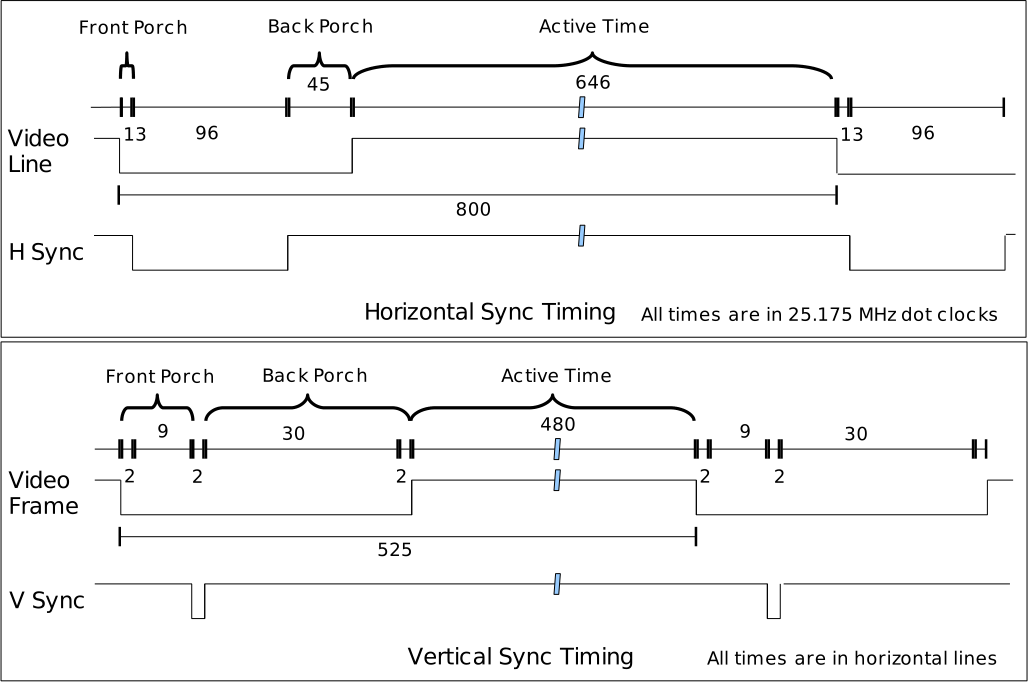
\includegraphics[scale=0.45]{images/vgatiming.png}
	\caption{Timings VGA \cite{cite:psocvga}}
	\label{fig:vgatiming}
\end{figure}

\noindent \textbf{N.B.} Les timings du tableau \cite{cite:timingsvga} et du schéma \cite{cite:psocvga} sont différents, ceux que nous avons choisis sont ceux du tableau.

\newpage
\subsection{Protocole PS/2 clavier}
Utilisant la DE0-Nano, nous souhaitions pouvoir avoir accès à des boutons supplémentaires et plus accessibles que sur la carte. Nous avons donc opté pour l'utilisation d'un clavier.\\

\begin{figure}[h!]
	\centering
	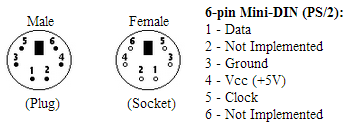
\includegraphics{images/ps2.png}
	\caption{6-pin Mini-DIN (PS/2) \cite{cite:ps2protocol}}
	\label{fig:ps2}
\end{figure}

Le connecteur PS/2 utilisé est un port mini-DIN possédant 6 broches (figure \ref{fig:ps2}). Celles qui nous intéressent sont la \emph{masse}, \emph{VCC (5V)}, \emph{Clock} et \emph{Data}. La ligne de données, \emph{Data}, est bidirectionnelle : le clavier peut communiquer avec le matériel connecté (envoie de données concernant les touches enfoncées) et inversement, nous n'utiliserons cependant que la communication clavier vers FPGA.\\

L'état par défaut des lignes \emph{Data} et \emph{Clock,} l'état d'attente, correspond à un 1 logique. Pour indiquer qu'une donnée est prête à être récupérée sur le signal \emph{Data}, le clavier met le signal \emph{Clock} à l'état bas. Les 8 bits de données peuvent ensuite être lus en série sur \emph{Data} sachant que le bit de poids faible sera envoyé en premier. Un bit de parité est ensuite envoyé, celui-ci permet la détection d'erreurs. Enfin, un bit de stop est envoyé pour indiquer la fin de la communication. Ci-dessous un récapitulatif des étapes de la communication clavier vers matériel.

\begin{enumerate}
\item 1 bit de \textbf{départ} : 0
\item 8 bits de \textbf{données}
\item 1 bit de \textbf{parité}
\item 1 bit de \textbf{fin} : 1\\
\end{enumerate}

% TODO parler du bit de parité

Le clavier envoie des \textbf{Scan codes}, ceux-ci permettent de représenter les différentes touches du clavier. Il existe deux types de codes: le premier type sert lors de l'appui sur une touche (make code), tandis que le second représente le relâchement d'une touche (break code). Un code peut comporter plusieurs octets, c'est le cas de la plupart des break codes. Le tableau suivant a été utilisé afin d'avoir la correspondance de chaque touche à ses codes: \href{http://www.computer-engineering.org/ps2keyboard/scancodes2.html}{http://www.computer-engineering.org/ps2keyboard/scancodes2.html}.\\
\textbf{N.B.} La correspondance entre touche et codes du tableau ci-dessus concerne les claviers QWERTY.\\

\newpage

\section{Implémentation}
\subsection{Environnement}
Nous avions au départ à notre disposition la Basys2 ainsi que le logiciel Xilinx et iSim pour visualiser les résultats de simulation. Afin de pouvoir avoir accès plus facilement à un FPGA et également profiter de plus de GPIOs et de mémoire nous avons acheté une DE0-Nano. Celle-ci étant un FPGA d'Altera, l'environnement de travail s'en est retrouvé changé. Nous sommes donc passé à Quartus pour le développement et la synthèse du code VHDL. De plus les IP cores diffèrent entre Xilinx et Quartus, nous avons donc dû effectuer quelques modifications au niveau de la ROM (utilisation du MegaWizard Manager de Quartus). Ayant rencontrés quelques problèmes avec Quartus, nous avons cependant continué à effectuer nos simulations à l'aide de Xilinx.\\

En ce qui concerne le matériel, nous avons utilisé une carte d'extension \cite{cite:vgaplus256kit} possédant entres autres un port VGA, un port PS/2 et un jack. La De0-Nano ne possédant pas de port VGA et de port PS/2, cela nous a permis d'interfacer un écran et un clavier à la carte.

\begin{figure}[h!]
	\centering
	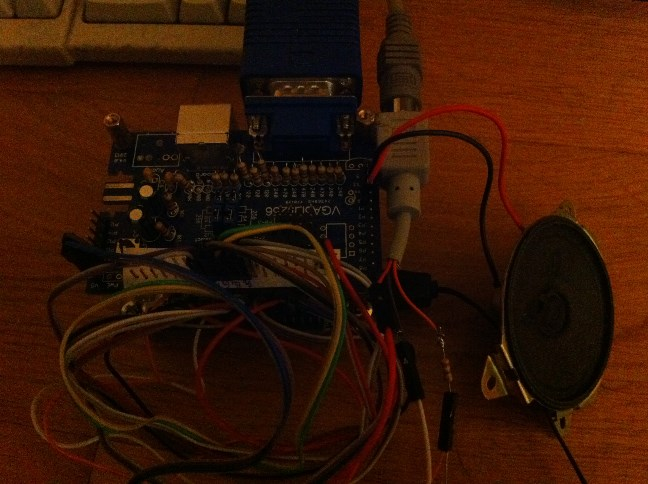
\includegraphics[scale=0.5]{images/IMG_1017.jpg}
	\caption{Photo de la DE0-Nano avec la carte d'extension fixée au dessus}
	\label{fig:photoDE0}
\end{figure}

\newpage
\subsection{Conventions}
Afin d'avoir une certaine cohérence entre nos différentes entités, nous avons essayé de respecter certaines conventions. Nous avons tout d'abord limiter l'utilisation de generics aux entités nécessitant de multiples instanciations, et d'utiliser des constantes contenus dans des packages (\emph{kbd\_pkg}, \emph{vga\_pkg}, \emph{game\_pkg}) dans les autres cas. Si nous avions utiliser des generics dans toutes les entités et avions seulement déclarés des constantes dans l'entité  \emph{pong} (top entity), nous aurions été forcé de cascader les generics ce qui devient vite contraignant.\\

Nous avons également utilisé \emph{open} afin de laisser vide des signaux de sorties dont nous ne nous servions pas lors d'instanciation d'entités. Pour les constantes et generics nous avons opté pour des majuscules, et pour les signaux des minuscules. les mots contenus dans les noms d'entités/signaux/constantes ont été séparés par des underscores ("\_"). De plus, lorsque cela était possible, nous avons utilisé la boucle \emph{for generate} afin de garder un code clair.

\newpage
\subsection{Génération signaux VGA}
\begin{figure}[h!]
	\centering
	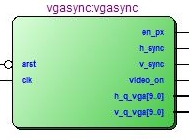
\includegraphics{images/vgasync.jpg}
	\caption{Schéma entité vgasync}
	\label{fig:vgasync}
\end{figure}

Ayant ajouté une carte d'extension utilisant des DACs 3 bits pour le rouge, 3 bits pour le vert, et 2 bits pour le bleu, nous avons généré nos couleurs sur 8 bits, soit 256 possibilités de couleurs. Nous avons également généré les signaux de synchronisation \emph{h\_sync} et \emph{v\_sync}.\\

D'après le tableau des timings du VGA\cite{cite:timingsvga}, pour une résolution de 640x480 60Hz la vitesse à laquelle doit être parcourue les pixels doit être d'environ 25 MHz. Pour cela nous avons instancié l'entité clkdiv ayant un enable (\emph{enclk}) en sortie permettant de faire fonctionner les autres blocs à une fréquence plus faible que celle de l'horloge.\\

Nous devons parcourir l'écran pixel par pixel, pour cela nous avons instancié deux compteurs (entité \emph{cnt}), un pour la position horizontale et l'autre pour la position verticale des pixels, comptant de 0 jusqu'à \emph{active zone} + \emph{back porch} + \emph{sync pulse} + \emph{front porch}. Ces compteurs sont autorisés à compter lorsque \emph{en\_px}  est à 1 (signal d'enable permettant de parcourir les pixels à 25 MHz). Lorsque le compteur horizontal arrive à sa valeur max, le signal \emph{maxed} du compteur passe à 1 et est relié à l'entrée \emph{cnten} du compteur vertical afin de l'autoriser à s'incrémenter, le compteur vertical s'incrémente donc à chaque fois qu'une ligne est parcourue.\\

Pour générer les signaux \emph{h\_sync} et \emph{v\_sync}, nous devons les mettre à l'état bas (actif) lorsque les compteurs \emph{h\_q\_int} et \emph{v\_q\_int} sont dans la zone de \emph{sync pulse}. Cela revient donc aux conditions suivantes :
\begin{flalign*}
&\text{\textbf{horizontal état bas (actif)}}&\\
&h\_q\_int >= H\_AT + H\_FP&\\
&\text{and } h\_q\_int < H\_AT + H\_FP + H\_SP&\\\\
&\text{\textbf{vertical état bas (actif)}}&\\
&v\_q\_int >= V\_AT + V\_FP&\\
&\text{and } v\_q\_int < V\_AT + V\_FP + V\_SP&
\end{flalign*}
Avec \emph{x\_q\_int} compteur de pixels \textbf{h}orizontal/\textbf{v}ertical\\
\emph{X\_AT} zone active horizontale/verticale\\
\emph{X\_FP} front porch horizontal/vertical\\
\emph{X\_BP} back porch horizontal/vertical\\
\emph{X\_SP} sync pulse horizontal/vertical\\

\newpage
Nous avons également généré un signal \emph{video\_on} actif lorsque les compteurs de pixels horizontal et vertical sont dans leur zone active respective.
\begin{flalign*}
&\text{\textbf{Conditions nécessaires pour \emph{video\_on} à l'état haut (actif)}}&\\
&h_q\_int < H\_AT&\\
&\text{and } v\_q\_int < V\_AT&
\end{flalign*}

\newpage
\subsection{Utilisation de la ROM}
La De0-Nano possède de la RAM utilisable à l'aide de blocs paramétrables dans Quartus II (Intellectual Property Blocks). L'outil MegaWizard Plug-In Manager (Tools -> MegaWizard Plug-In Manager) permet de créer des entités donnant accès à différents types de mémoires (RAM: 1-PORT, ROM:1-PORT, etc).\\

\begin{figure}[h!]
	\centering
	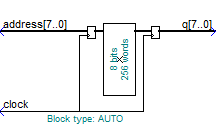
\includegraphics{images/romschem.png}
	\caption{Schéma ROM contenant 256 adresses et 8 bits de sortie}
	\label{fig:romschem}
\end{figure}

Nous souhaitons créer une ROM: 1-PORT contenant des images à afficher sur l'écran. Celle-ci comporte 2 entrées, horloge et adresse, et une sortie. La taille du bus d'adresse et de sortie doivent être précisées. La dernière étape est l'indication d'un fichier \emph{mif} décrivant le contenu de la ROM. Celle-ci nécessite les informations suivantes :
\begin{description}
\item[Depth] indique la taille du bus d'adresses
\item[Width] indique la taille du bus de sortie
\item[Address radix] base utilisée pour les adresses
\item[Data radix] base utilisée pour les données
\item[Content] Contenu de la ROM sous la forme \emph{adresse : donnée;}
\end{description}

Nous avons généré deux ROMs, l'une contenant un jeu de caractère (noir et blanc), et l'autre contenant une image à afficher en fond ($95*128$, 8 bits de couleurs). Pour générer le fichier \emph{mif} correspondant à ces images, une fonction MATLAB \cite{cite:rommatlab} a été utilisée pour générer un fichier \emph{mif}, puis un traitement simple a été effectué pour rajouter des adresses associées à la donnée \emph{0x00} afin d'atteindre une puissance de 2.\\

\noindent \textbf{N.B.} Le code ci-dessous correspond à la fonction permettant de convertir une image ayant des couleurs sur 8 bits. Pour une image ne possédant qu'un seul bit de couleur (noir ou blanc) la fonction a été modifiée.\\

\begin{lstlisting}
function img2 = IMG2mif8(imgfile, outfile)

img = imread(imgfile);
height = size(img, 1);
width = size(img, 2);
s = fopen(outfile,'wb');

% header
fprintf(s,'DEPTH = %d;\n', height*width);
fprintf(s,'WIDTH = 8;\n');
fprintf(s,'ADDRESS_RADIX = UNS;\n');
fprintf(s,'DATA_RADIX = HEX;\n');
fprintf(s,'CONTENT\n');
fprintf(s,'BEGIN\n');

% content
cnt = 0;
cntadr = 0;
img2 = img;
for r=1:height
    for c=1:width
        cnt = cnt + 1;
        R = img(r,c,1);
        G = img(r,c,2);
        B = img(r,c,3);
        Rb = dec2bin(R,8);
        Gb = dec2bin(G,8);
        Bb = dec2bin(B,8);
        img2(r,c,1) = bin2dec([Rb(1:3) '00000']);
        img2(r,c,2) = bin2dec([Gb(1:3) '00000']);
        img2(r,c,3) = bin2dec([Bb(1:2) '000000']);
        Outbyte = [ Rb(1:3) Gb(1:3) Bb(1:2) ];
        if (Outbyte(1:4) == '0000')
            fprintf(s,'%d : 0%X',cntadr, bin2dec(Outbyte));
        else
            fprintf(s,'%d : %X',cntadr, bin2dec(Outbyte));
        end
        
        fprintf(s,';\n');
        cntadr = cntadr + 1;
    end
end

fprintf(s,'END;');

fclose(s);
\end{lstlisting}

\begin{figure}[h!]
	\centering
	\begin{subfigure}[b]{0.1\textwidth}
		\centering
		
\includegraphics[width=\textwidth]{images/cirno2.jpg}
		\label{fig:cirno2}
	\end{subfigure}
	~

	\begin{subfigure}[b]{0.4\textwidth}
		\centering
		
\includegraphics[width=\textwidth]{images/pixelfont.jpg}
		\label{fig:pixelfont}
	\end{subfigure}
	\caption{Images contenues dans la ROM}
\end{figure}


\begin{figure}[h!]
	\centering
	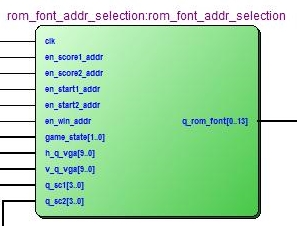
\includegraphics[scale=1.0]{images/romfontaddr.jpg}
	\caption{Schéma entité rom\_font\_addr\_selection}
	\label{fig:romfontaddr}
\end{figure}
La sélection d'adresses pour la ROM contenant le jeu de caractères se fait au niveau de l'entité \emph{rom\_font\_addr\_selection}. Celle-ci prend en entrée un enable pour les différentes zones dans lesquelles le contenu de la ROM doit être affiché. Cette enable doit se produire un cycle d'horloge avant l'affichage dans la zone désirée, en effet le bloc de ROM dépend de l'horloge, et lorsqu'une adresse entre dans celui-ci la sortie est disponible au coup d'horloge suivant.\\

Une fois l'adresse sélectionnée, pour récupérer la sortie nous pouvons utiliser le compteur de position horizontal (valeur du compteur horizontal - position horizontale du caractère à afficher), ce qui nous permet de récupérer les bits un par un afin de définir ou non une couleur spécifique pour le pixel actuellement parcouru.\\

Pour générer l'image de fond, le principe diffère légèrement. En effet pour une adresse donnée, la sortie de \emph{rom\_bg} est la couleur d'un pixel. Pour adresser chaque pixel il faudrait donc multiplier les deux signaux de compteurs de pixels (horizontal et vertical). Pour éviter cela, un compteur supplémentaire a été crée afin de compter à la vitesse de la pixel clock lorsque les compteur de pixels se trouvent dans la bonne zone.

\newpage
\subsection{Utilisation du clavier}
\begin{figure}[h!]
	\centering
	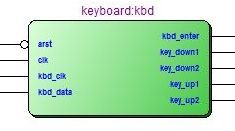
\includegraphics[scale=1.0]{images/kbdentity.jpg}
	\caption{Schéma entité keyboard}
	\label{fig:kbdentity}
\end{figure}

La gestion du clavier se fait à l'aide de l'entité \emph{keyboard}. Celle-ci prend en entrée les signaux \emph{kbd\_clk}, signal d'enable généré par le clavier permettant d'indiquer lorsqu'une donnée est reçue, et \emph{kbd\_data}, signal permettant de recevoir les données en série. Les signaux de sortie indiquent l'état d'une touche du clavier, \emph{key\_up1}, \emph{key\_down1}, \emph{key\_up2}, \emph{key\_down2} et \emph{key\_enter} correspondant respectivement aux touches A, Q, Z, S et ENTRÉE du clavier.\\

Lorsqu'une donnée est disponible sur le signal \emph{kbd\_data}, le signal \emph{kbd\_clk} passe à l'état bas (actif). Nous devons donc détecter un front descendant sur ce dernier en comparant sa valeur actuelle et son ancienne valeur \emph{kbd\_clk\_old}. Pour cela nous assignons la valeur de \emph{kbd\_clk} à \emph{kbd\_clk\_old} lorsqu'un coup d'horloge intervient. Les données sont ensuite récupérées une par une à l'aide d'un registre à décalages Serial-In Parallel-Out, \emph{data\_shift}. Les 8 bits de données peuvent être récupérés sur le signal \emph{data} lorsque le bit de start atteint le LSB de \emph{data\_shift} (initialement rempli de '1'). Une fois une donnée disponible, celle-ci est comparée aux codes correspondant aux touches qui nous intéressent pour savoir si le signal correspondant doit passer à l'état actif ou non. Pour vérifier le relâchement d'une touche, l'ancienne valeur contenue dans data est stockée dans \emph{old\_data}, ce qui permet de vérifier si le code relâchement a été envoyé et avec quel code de touche celui-ci a été envoyé.

\newpage

\section{Intégration du jeu}
\subsection{Jeu}
\begin{figure}[h!]
	\centering
	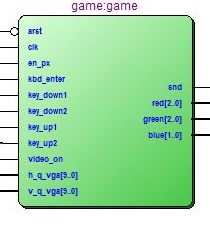
\includegraphics[scale=1.0]{images/game.jpg}
	\caption{Entité game}
	\label{fig:game}
\end{figure}
L'entité \emph{game} a pour rôle d'instancier tous les éléments nécessaires au jeu. L'entité \emph{clkdiv} est instancié pour obtenir un enable permettant de gérer la vitesse de mise à jour du jeu en lui même, et un autre enable pour gérer la vitesse des raquettes uniquement. Les autres entités instanciées sont les suivantes \emph{player} (gestion du joueur), \emph{sounds} (génération des sons de collision), \emph{ball} (gestion de la balle), \emph{score}, \emph{game\_gen} (génération des éléments du jeu via les signaux de couleurs du VGA), \emph{game\_state} (état du jeu).
\begin{figure}[h!]
	\centering
	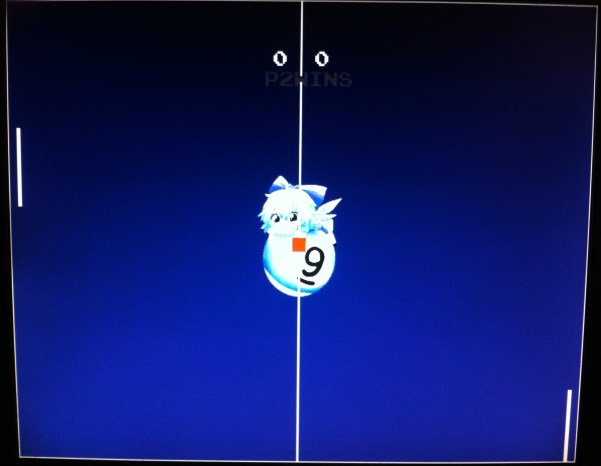
\includegraphics[scale=0.5]{images/IMG_1015.jpg}
	\caption{Photo du jeu en fonctionnement}
	\label{fig:photogame}
\end{figure}

\newpage
\subsection{Éléments du jeu}
\begin{figure}[h!]
	\centering
	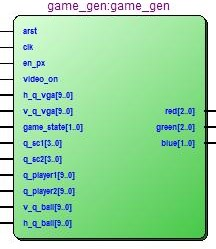
\includegraphics[scale=1.0]{images/gamegen.jpg}
	\caption{Entité game\_gen}
	\label{fig:gamegen}
\end{figure}

La génération des éléments du jeu et des couleurs s'effectue grâce à l'entité \emph{game\_gen}. Celle-ci possède en sortie les 3 signaux de couleurs nécessaires à l'affichage VGA \emph{red}, \emph{green} et \emph{blue}. Les entrées sont principalement les différents compteurs de position (\emph{h\_x\_vga},  \emph{q\_scx}, \emph{q\_player1} et \emph{x\_q\_ball}.\\

Le signal \emph{color\_gen} permet de coder la priorité d'affichage des différents éléments du jeu. Les éléments à afficher sont les suivants (du plus important au moins important) :
\begin{description}
\item[win\_gen] texte "P1/2WINS"
\item[start\_gen] texte "PRESS ENTER"
\item[ball\_gen] balle
\item[player\_gen] joueur
\item[score2\_gen] affichage score joueur2
\item[score1\_gen] affichage score joueur1
\item[bg\_gen] affichage background
\item[BLACK] affichage couleur noire (lorsque les compteurs de pixels ne sont plus dans la zone active définie par \emph{video\_on})
\end{description}

\newpage
\subsection{État du jeu}
\begin{figure}[h!]
	\centering
	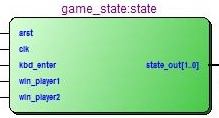
\includegraphics[scale=1.0]{images/gamestate.jpg}
	\caption{Entité game\_state}
	\label{fig:gamestate}
\end{figure}
La gestion de l'état dans lequel se trouve le jeu se trouve dans l'entité \emph{game\_state}. Celle-ci est une machine
d'état décrite par le schéma suivant (\emph{game\_state} état actuel de la machine d'état, \emph{kbd\_enter\_new} état actuel de la touche entrée du clavier, \emph{kbd\_enter\_old} ancien état de la touche entrée du clavier, \emph{win\_player1} état de victoire du joueur 1, \emph{win\_player2} état de victoire du joueur 2):
\begin{figure}[h!]
	\centering
	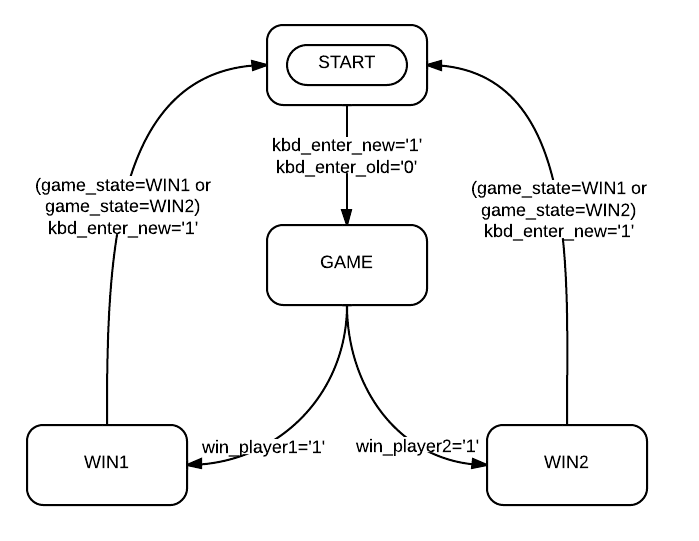
\includegraphics[scale=0.5]{images/BasicStateDiagram.png}
	\caption{Schéma de la machine d'état}
	\label{fig:statemachine}
\end{figure}

Les états possibles sont les suivants :
\begin{description}
\item[START] Affichage du texte "PRESS START", attente de l'appui sur la touche entrée pour lancer le jeu
\item[GAME] Jeu en fonctionnement
\item[WIN1] Le player1 a gagné, affichage du texte "P1WINS", attente de l'appui sur la touche entrée pour revenir à l'écran start
\item[WIN2] le player2 a gagné, affichage du texte "P2WINS", attente de l'appui sur la touche entrée pour revenir à l'écran start
\end{description}

\newpage
\subsection{Joueur}
\begin{figure}[h!]
	\centering
	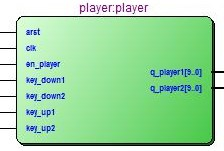
\includegraphics[scale=1.0]{images/player.jpg}
	\caption{Entité player}
	\label{fig:player}
\end{figure}

Un joueur est représenté par sa raquette. La gestion des joueurs est effectuée dans l'entité \emph{player} qui contient un compteur de position verticale pour chaque joueur. Ce compteur (instanciation de l'entité \emph{cnt\_player}) peut compter de 0 (haut de l'écran) jusqu'à \emph{zone active verticale} - \emph{hauteur du joueur} (bas de l'écran).\\

\begin{figure}[h!]
	\centering
	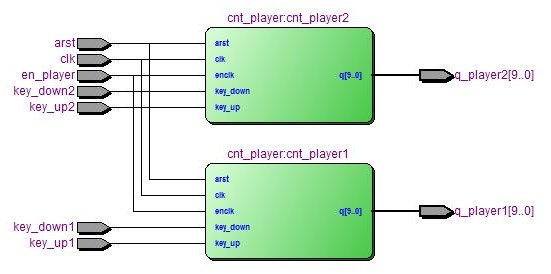
\includegraphics[scale=1.0]{images/player_player.jpg}
	\caption{Schéma interne de l'entité player}
	\label{fig:playerplayer}
\end{figure}

L'entité \emph{cnt\_player} gérant la position d'un joueur est un compteur pouvant s'incrémenter ou se décrémenter en fonction des signaux \emph{key\_up} et \emph{key\_down}. Ces signaux proviennent de l'état de boutons contrôlant les raquettes des joueurs, boutons provenant dans notre cas du clavier interfacé avec le FPGA. Si la valeur maximum(ou minimum) du compteur est atteinte, le compteur reste à cette valeur si le signal \emph{key\_down} (ou \emph{key\_up}) est actif.\\

L'entité \emph{player} possède en sortie les signaux \emph{q\_player1} et \emph{q\_player2} provenant des compteurs de position des joueurs.

\newpage
\subsection{Balle}
\begin{figure}[h!]
	\centering
	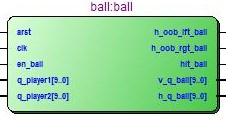
\includegraphics[scale=1.0]{images/ball.jpg}
	\caption{Entité ball}
	\label{fig:ball}
\end{figure}

La balle est le seul élément du jeu à se déplacer en deux dimensions. Sa gestion est effectuée dans l'entité \emph{ball} et  fait appel à trois paramètres : position, vitesse et angle de déplacement. Dans les premières versions du projet, la position était le seul paramètre variable (valeurs des compteurs de position). Par la suite, la vitesse et l'angle de déplacement sont devenus des variables.\\

Comme la balle se déplace en deux dimensions, il a fallu trouver un système permettant de gérer les déplacements horizontaux et verticaux simultanément. Les compteurs se sont immédiatement imposés comme le meilleur moyen de gérer une position, leurs valeurs respectives donnant la position de la balle a un instant précis. La position future de la balle dépend de sa position actuelle et de différents paramètres, notamment le choc contre une raquette ou la sortie de l'écran ou encore le fait que la balle soit montante ou descendante. Les compteurs devaient donc adapter leur comportement en fonction de ces paramètres.\\

Au départ, il s'agissait de deux compteurs basiques à deux modes : incrémentation et  décrémentation. Leurs comportements étant différents ils possédaient deux architectures différentes : une pour la position horizontale et une pour la position verticale. Dans la dernière version il s'agit toujours d'un compteur à deux modes, l'entité \emph{cnt\_ball}, cependant le mode de fonctionnement (horizontal ou vertical) n'est plus géré par deux architectures différentes mais par un generic, \emph{CNT\_MODE} (peut prendre les valeurs (\emph{CNT\_MODE\_H} ou \emph{CNT\_MODE\_V}. Ce compteur est instancié deux fois, une pour la position horizontale de la balle, et l'autre pour la position verticale.\\

Les génériques MAX et MIN permettent de définir les valeurs extrêmes prises par q, sortie du compteur. Il faut garder à l'esprit que du fait de la multiple instanciation, les valeurs de MAX et de MIN sont définies différemment selon le mode du compteur : vertical ou horizontal.\\

Le signal \emph{mode} dans \emph{cnt\_ball} permet de contrôler le sens de variation des compteurs : incrémentation ou décrémentation. Le \emph{spd\_mod} permet de contrôler la vitesse du compteur : selon sa valeur le compteur est incrémenté ou décrémenté, d'une valeur plus ou moins élevé.\\

L'angle de rebond n'est pas une variabe, il est calculé grâce à un système de zone de collision et appliqué grâce à une combinaison des \emph{spd\_mod} sur les compteurs verticaux et horizontaux. Le comportement de la balle dépend de l'endroit où elle touche la raquette. Pour cela, on utilise les signaux \emph{hit\_rgt\_area} et \emph{hit\_left\_area} qui influe sur le comportement de \emph{spd\_mod}. Ces signaux sont des entrées de l'entité, ils sont générés dans l'entité \emph{ball}.\\

\newpage
\begin{figure}[h!]
	\centering
	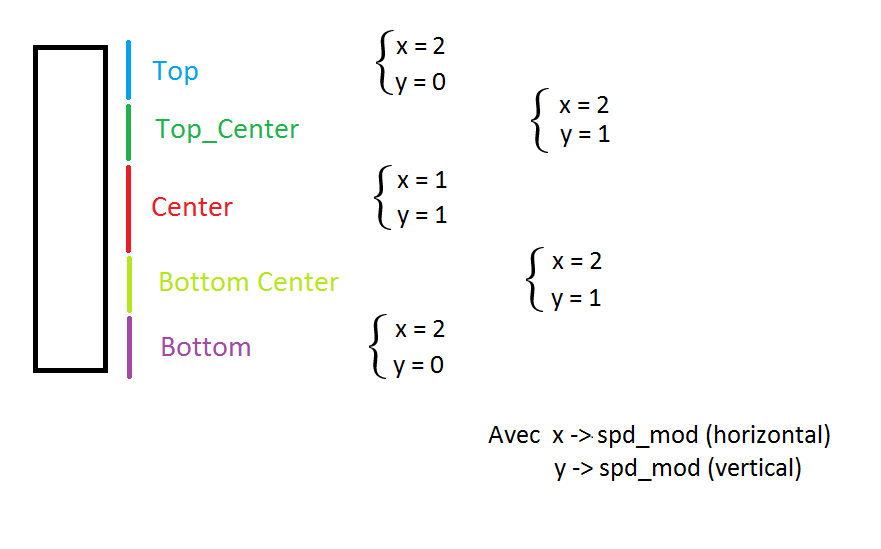
\includegraphics[scale=0.5]{images/collisions.png}
	\caption{Schéma zones de collision et effets sur la balle}
	\label{fig:collisions}
\end{figure}

Les signaux \emph{oob\_rgt} et \emph{oob\_lft} sont utilisés afin de savoir si la balle est sortie de l'écran horizontalement et permet donc de savoir si un des joueurs à marqué un point.

\newpage
\subsection{Scores}
\begin{figure}[h!]
	\centering
	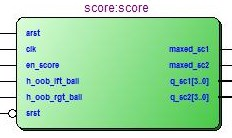
\includegraphics[scale=1.0]{images/score.jpg}
	\caption{Entité score}
	\label{fig:score}
\end{figure}

La gestion des scores est effectuée dans l'entité \emph{score} qui possède en entrée le signal d'enable \emph{en\_score} (vitesse de mise à jour du jeu), des signaux permettant de savoir si la balle est sortie de l'écran à droite ou à gauche \emph{h\_oob\_rgt\_ball} et \emph{h\_oob\_lft\_ball}. Les sorties sont des vecteurs permettant de connaître le score \emph{q\_sc1} et \emph{q\_sc2}, et deux signaux permettant de savoir si le score a atteint sa valeur max \emph{maxed\_sc1} et \emph{maxed\_sc2}.\\

\begin{figure}[h!]
	\centering
	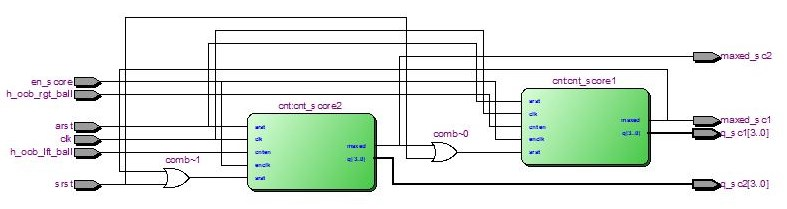
\includegraphics[scale=0.75]{images/scorein.jpg}
	\caption{Schéma interne de l'entité score}
	\label{fig:scorein}
\end{figure}
L'architecture de cette entité contient l'instanciation de deux compteurs (entité \emph{cnt}) permettant de compter de 0 jusqu'à \emph{MAX\_SCORE}. Ces compteurs sont autorisés à compter lorsque le joueur correspondant à marqué un point (\emph{h\_oob\_rgt\_ball} à l'état haut ou \emph{h\_oob\_lft\_ball} à l'état haut). Enfin, le reset synchrone des compteurs est activé lorsqu'un des joueurs à atteint le score max et/ou que le jeu n'est pas dans l'état \emph{GAME} (voir partie sur la gestion des états du jeu).

\newpage
\subsection{Génération de sons}
\begin{figure}[h!]
	\centering
	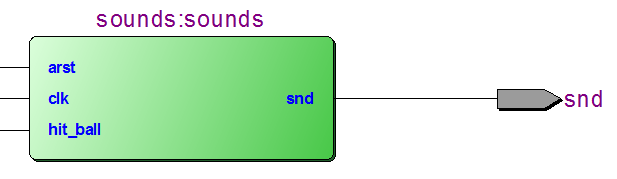
\includegraphics[scale=0.75]{images/soundsschem.png}
	\caption{Schéma entité sounds}
	\label{fig:soundschem}
\end{figure}

Le haut parleur que nous utilisons possède une impédance de 8 Ohms et une puissance maximale de 0.3W. Nous sortons du 3.3V LVTTL avec un courant de 8 mA sur le pin sur lequel nous branchons le haut-parleur.\\

Pour générer un son, nous devons envoyer un signal périodique possédant une fréquence contenue dans les fréquences audibles au haut-parleur. Pour ce faire nous avons instancié l'entité \emph{clkdiv} afin de générer un \emph{enable} permettant de faire fonctionner d'autres signaux à une certaine fréquence. Soit \emph{BUMP\_SOUND}, fréquence souhaitée en utilisant le diviseur d'horloge. Le son est généré en inversant l'état du signal \emph{bumpsnd} à chaque impulsion \emph{enable}, la fréquence sortie sera donc le double de celle précisée dans la constant \emph{BUMP\_SOUND}.\\

Une fois le son généré, nous souhaitons pouvoir le maintenir, pour cela nous utilisons un autre diviseur d'horloge utilisant une fréquence \emph{HOLD\_SOUND}, dont la période correspondante est le temps de maintien du son. Nous autorisons ensuite à sortir le signal \emph{bumpsnd} de l'entité lorsqu'une collision entre la balle et une raquette intervient (\emph{hold\_hit\_ball}='1') et tant que l'enable du diviseur d'horloge de maintien du son ne passe pas à l'état bas.

\begin{figure}[h!]
	\centering
	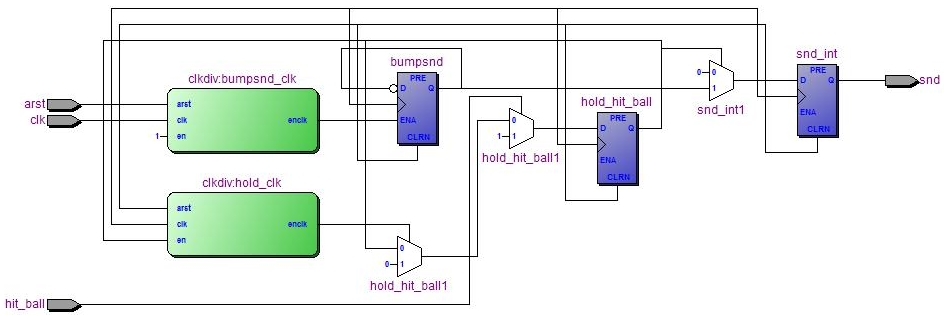
\includegraphics[scale=0.70]{images/soundsschem2.jpg}
	\caption{Schéma interne entité sounds}
	\label{fig:soundschem2}
\end{figure}

\newpage

\section{Conclusion}
Ce projet nous a permis de renforcer les bases acquises en VHDL durant l'unité du premier semestre et d'acquérir de nouvelles connaissances en interfaçant des périphériques que nous n'avions pas utilisé en TP.
La majeure partie des objectifs a été remplie, le jeu, les sons et le clavier étant fonctionnels. Des difficultés ont été rencontrées d'un point de vue matériel (problèmes apparaissant avec le clavier corrigés en mettant des résistances en série sur les fils kbd\_data et kbd\_clk) et d'un point de vue développement (collisions, adressage ROM, ...). Si nous avons atteint tous les objectifs, nous pensons cependant pouvoir améliorer notre future gestion de projet grâce à github qui nous aurait permis de mieux répartir le travail.

\newpage


\begin{thebibliography}{10}
\bibitem{cite:pong} Jean Zeid, \emph{Jeux vidéo : de Pong (1972) aux jeux 3D}, \href{http://www.franceinfo.fr/education-jeunesse-jeux-video/jeux-video-de-pong-1972-aux-jeux-3d-439411-2011-11-07}{http://www.franceinfo.fr/education-jeunesse-jeux-video/jeux-video-de-pong-1972-aux-jeux-3d-439411-2011-11-07}

\bibitem{cite:ps2protocol}  Adam Chapweske, \emph{The PS/2 Mouse/Keyboard Protocol}, \href{http://www.computer-engineering.org/ps2protocol/}{http://www.computer-engineering. org/ps2protocol/}

\bibitem{cite:howtvworks} Marshall Brain, \emph{How Television Works}, How stuff works, \href{http://electronics.howstuffworks.com/tv7.htm}{http://electronics.howstuffworks.com/tv7.htm}

\bibitem{cite:simplevga} Dave Vandenbout, \emph{A Simple VGA Interface for the XuLA FPGA Board}, \href{http://devbisme.webfactional.com/blogs/devbisme/2011/06/02/simple-vga-interface-xula-fpga-board}{http://devbisme.webfactional.com/blogs/devbisme/2011/06/02/simple-vga-interface-xula-fpga-board}

\bibitem{cite:timingsvga} \emph{VGA Signal 640 x 480 @ 60 Hz Industry standard timing} , TinyVGA, \href{http://tinyvga.com/vga-timing/640x480@60Hz}{http://tinyvga.com/vga-timing/640x480@60Hz}

\bibitem{cite:psocvga} Mac A. Cody, \emph{Driving A VGA Display With A Cypress PSoC}, \href{http://home.roadrunner.com/~maccody/PSoC/VGA/PSoC\_VGA\_Driver.html}{http://home.roadrunner.com/~maccody/PSoC/VGA/PSoC\_VGA\_Driver.html}

\bibitem{cite:vgapinout} \emph{VGA Pinout} \href{http://www.teletechsvc.net/pinouts/db15-vga-pinout.html}{http://www.teletechsvc.net/pinouts/db15-vga-pinout.html}

\bibitem{cite:scan} Bryan Ackland, \emph{Lab 3: VGA Bouncing Ball I}, \href{http://personal.stevens.edu/~backland/Courses/Course487\_Spring_13\_files/Labs/Lab3.pdf}{http://personal.stevens.edu/~backland/Courses/Course487\_Spring\_13\_files/Labs/Lab3.pdf}

\bibitem{cite:rommatlab} \emph{Sprites in Block ROM}, \href{http://www.lbebooks.com/downloads/exportal/VHDL\_NEXYS\_Example24.pdf}{http://www.lbebooks.com/downloads/exportal/VHDL\_NEXYS\_Example24.pdf}

\bibitem{cite:vgaplus256kit} \emph{VGAplus256 Kit}, \href{http://propellerpowered.us/index.php?route=product/product\&product\_id=62}
{http://propellerpowered.us/index.php?route=product/product\&product\_id=62}

\end{thebibliography}

\end{document}
